\subsection{Alloy Code}
This section is dedicated to the Alloy model of the CLup  software, included all the functions of the application and their most important constraints.\\
In the model are represented the two categories of users: the store owners and the customers. Each store owner owns a set of stores, and each customer opens a set of reservations. Those reservations can be of three types: immediate, on premise and future. Every reservation refers to a store, has an estimated time for the customer who opened it to reach the store, a time for that customer to wait before he/she is able to enter, a value representing in which moment the reservation has been created, and a boolean value, representing whether the customer has already been alerted (he/she must depart to reach the store). Moreover each reservation can be in one of 4 states:
\begin{itemize}
	\item PENDING: reservation has been requested but customer cannot yet access the store
	\item AUTHORIZED: customer can access the store for a time window
	\item CURRENT: customer has accessed the store and has not exited yet
	\item EXPIRED: customer has exited the store or the time window to enter the store ended or the reservation was deleted
\end{itemize}
Finally a future reservation keeps track of entry time.

We apply some constraints to the model so that it can represent the application domain of our S2B.\\
First, customers are queued up following a First In First Out policy. We ensure that the parameters in the reservations are meaningful with respect to the state of the reservation itself, e.g. a customer is alerted when the time remaining before it is his/her turn is less or equal than the time for him/her to reach the store. For every store we check that the current occupation is equal to the number of customer inside the store and that this value never exceeds the maximum occupation of that store.

\lstinputlisting[language=alloy]{alloy.als}
\newpage
\subsection{Scenarios}
Those are some instances of the Alloy model based on the predicates above.
\begin{flushleft}
	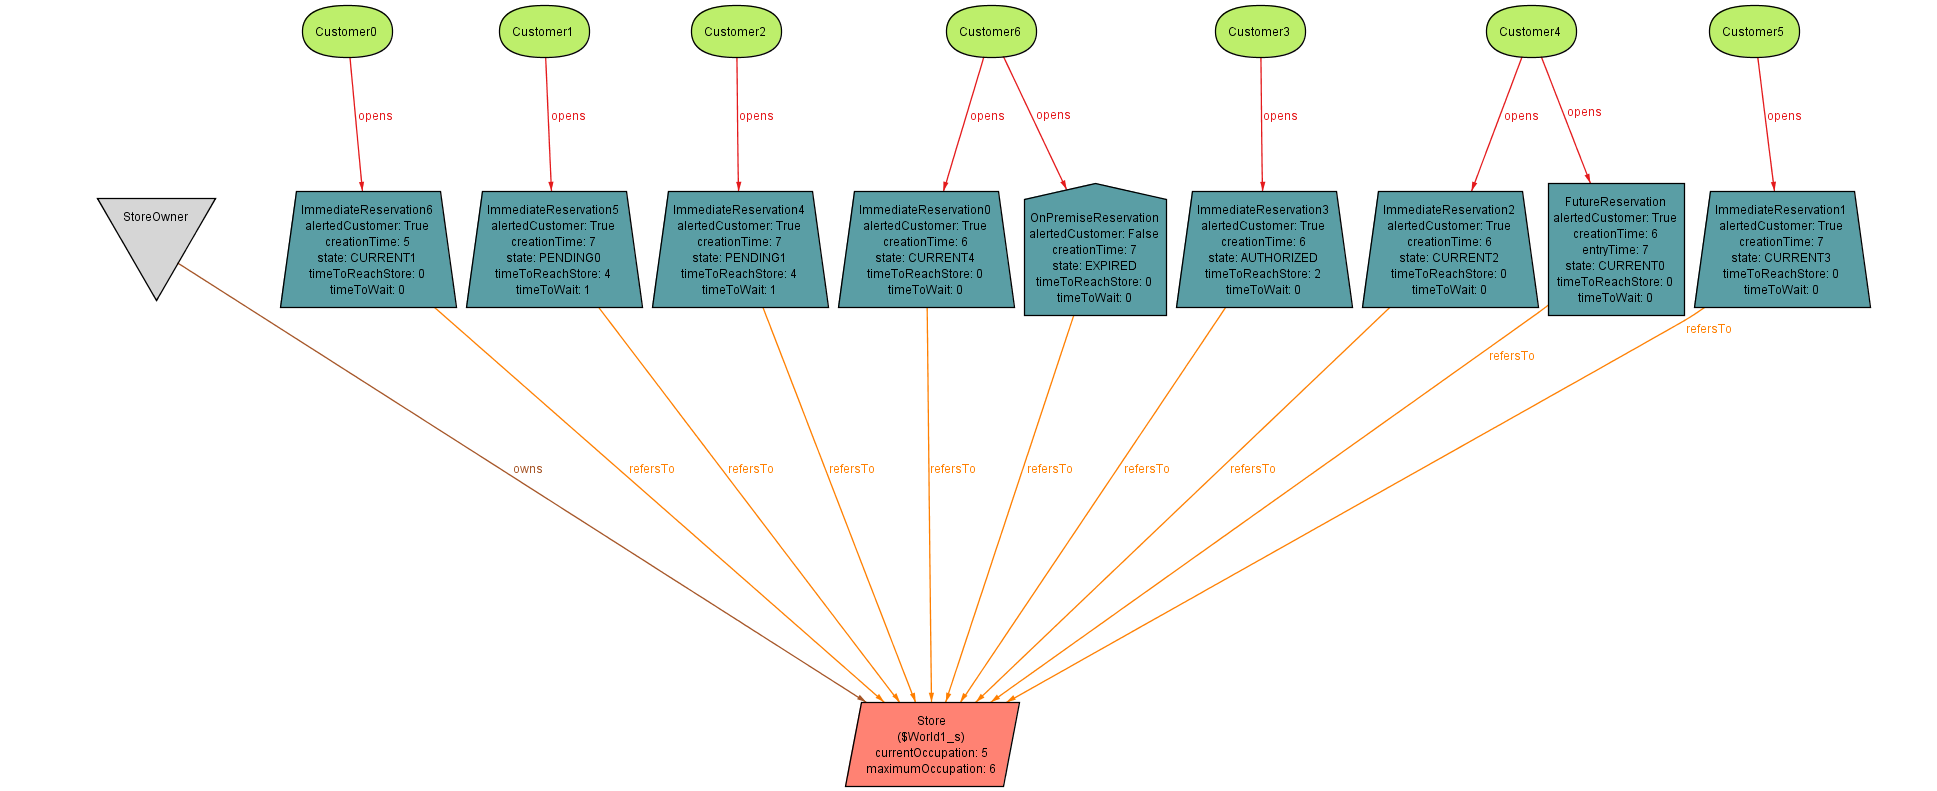
\includegraphics[scale=0.25]{Images/Alloy_World1.png}
\end{flushleft}
The first scenario shows a store with a current occupation of 5, which represents the actual number of current reservations, and we observe that it is still less than the maximum occupation.\\\\

\begin{flushleft}
	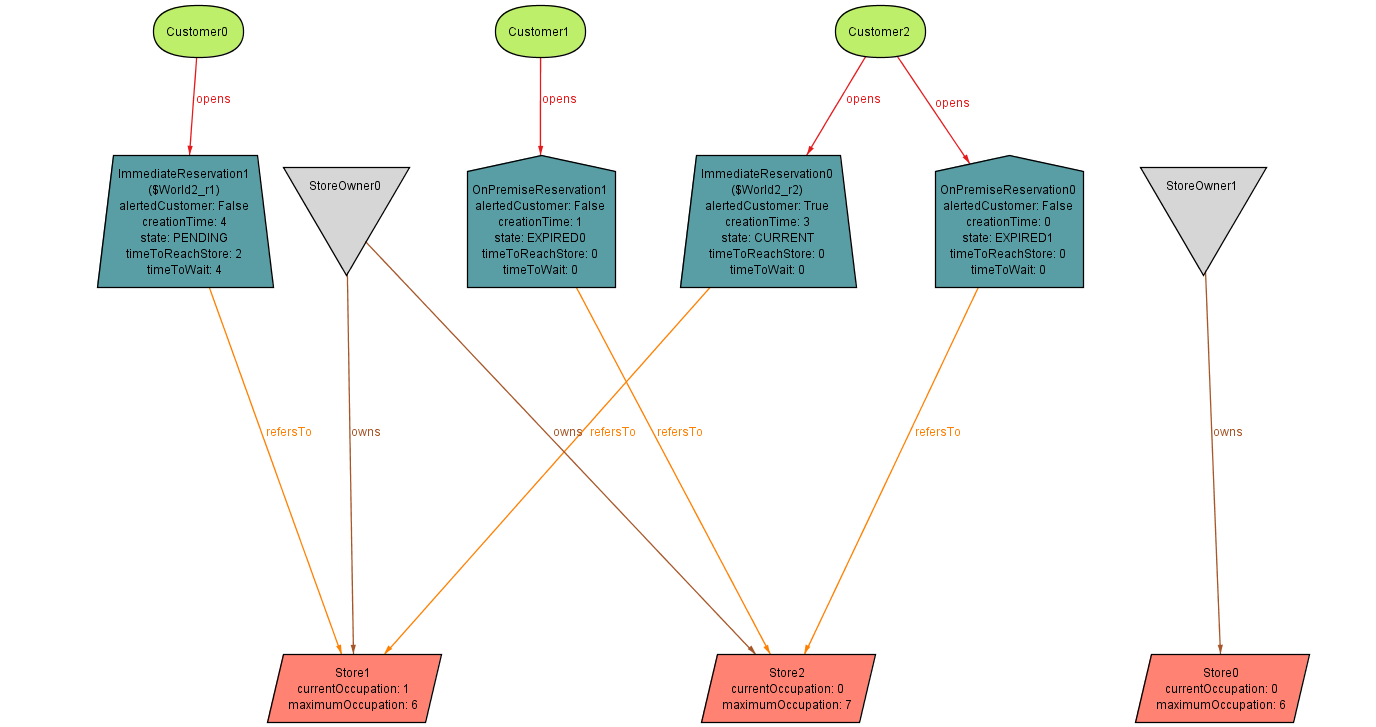
\includegraphics[scale=0.3]{Images/Alloy_World2.png}
\end{flushleft}
In the second scenario there are two immediate reservations r1 and r2 for the same store. r1 has been created after r2, so r2 has less time to wait with respect to r1.\\
Moreover the customer that opened r2 has been alerted because his time to wait is less or equal than the time for him to reach the store, while for r1 this property doesn't hold, so the customer has not been alerted.\\\\

\begin{flushleft}
	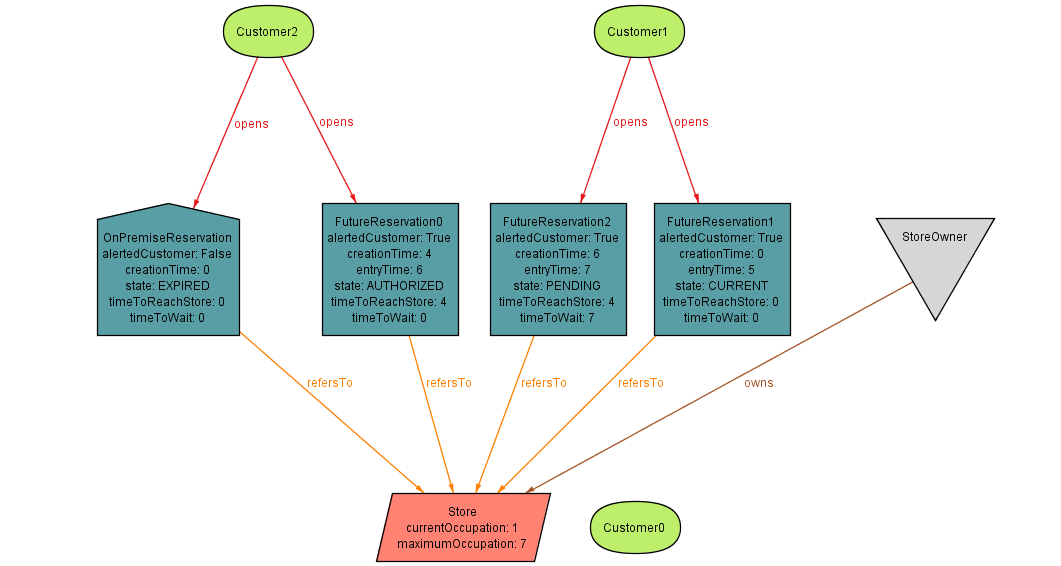
\includegraphics[scale=0.4]{Images/Alloy_World3.png}
\end{flushleft}
In the third scenario there is a customer which has not opened any reservation yet.\\
Customer 1 has booked two reservations and they have different entry time.\\\\

\begin{flushleft}
	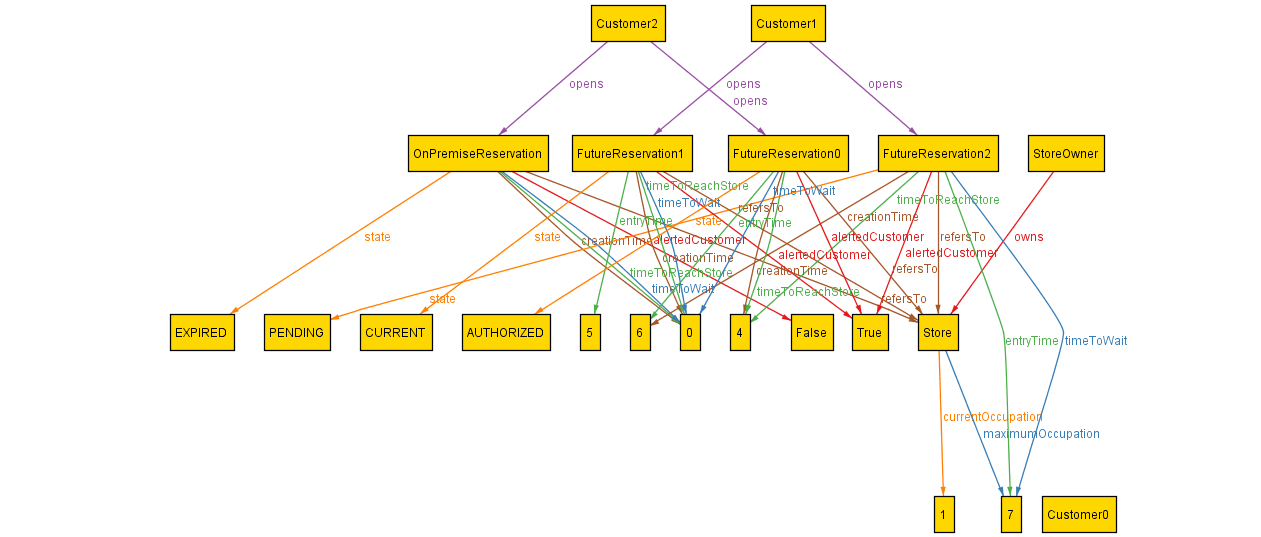
\includegraphics[scale=0.4]{Images/Alloy_World3_ugly.png}
\end{flushleft}
We used a theme in the diagrams above to make them more readable; without the theme the third diagram would look like this.



